\documentclass{article}
\usepackage{fullpage}
\usepackage{pgf-pie}
\usepackage[utf8]{inputenc}
\usepackage{multicol} 
\usepackage[a4paper, total={6in, 8in}]{geometry}
\usepackage{amsmath}
\usepackage{adjustbox}

\usepackage{tabulary}
\usepackage{booktabs}
\usepackage{pgfplots}
\usepackage{float}
\usepackage{tabularx,ragged2e,booktabs,caption}
\newcolumntype{C}[1]{>{\Centering}m{#1}}
\renewcommand\tabularxcolumn[1]{C{#1}}
\pgfplotsset{compat=1.8}
\usepgfplotslibrary{statistics}


\title{Flight Delay Prediction}
\author{Rishi Vardhan K}

\begin{document}

\maketitle

\begin{abstract}
\textbf{
Flight delay is when an airline flight takes off and/or lands later than its scheduled time. Several factors affect flight delay with respect to weather parameters and management errors. The project works with real time weather data on a two stage predictive machine learning engine that predicts the chance of a flight to be delayed and the amount of delay.
}
\end{abstract}

\section{Introduction}

Flight delays are an important factor to consider whilst flight operation. There are factors that are under the direct control of the carrier, such as aircraft turnarounds between flights, passenger punctuality, technical and crew performance, etc. There are also even more factors that are outside of the airline’s control, such as weather, air traffic control, security, airport conditions, etc. The reality is such that so long as airplanes continue flying, flight delays will be a part of the experience. According to the Bureau of Statistics, about 20\%\ of all flights are delayed by 15 minutes or more. \\

As flight delays are caused by either of factors affecting departure or arrival, the project works on dealing with predicting and calculating delay pertaining to arrival of flight. The project is divided into three modules each with different sets of operations. Module 1 focuses on Data Pre-processing, Module 2 on Classification and Module 3 on Regression. Each Module works incrementally on previous module's output. 
\section{Data Pre-Processing - Module 1}
The first module operates to process the data to fit under the required problem statement. The flight data is obtained from the Bureau of Transportation Statistics between years 2016-2017. The corresponding weather data for the years is also collected. Each data-set is filtered to contain features with maximum relevance to the given problem. The following are the list of airport codes considered for the model. The data is processed so as to work with arrival and departure of flights only under these airports.
\begin{center}
\captionof{table}{Airport Codes} \label{tab:title} 
\begin{tabular}{ |c|c|c| } 
 \hline
 ATL & CLT & DEN \\ 
 \hline
 DFW & EWR & IAH \\
 \hline
 JFK & LAS & LAX \\
 \hline
 MCO & MIA & ORD \\
 \hline
 PHX & SEA & SFO \\ 
 \hline
\end{tabular}
\end{center}

The following are the features considered from real-time weather data-set.
\begin{center}
\captionof{table}{Weather Features} \label{tab:title} 
\begin{tabular}{ |c|c|c| } 
 \hline
 WindSpeedKmph & WindDirDegree & WeatherCode \\ 
 \hline
 precipMM & Visiblity & Pressure \\
 \hline
 Cloudcover & DewPointF & WindGustKmph \\
 \hline
 tempF & WindChillF & Humidity \\
 \hline
 date & time & airport \\ 
 \hline
\end{tabular}
\end{center}

The following are the features considered from real-time flight performance data-set.

\begin{center}
\captionof{table}{Flight Features} \label{tab:title} 

\begin{tabular}{ |c|c|c| } 
 \hline
 FlightDate & Quarter & Year \\ 
 \hline
 Month & DayofMonth & DepTime \\
 \hline
 DepDel15 & CRSDepTime & DepDelayMinutes \\
 \hline
 OriginAirportID & DestAirportID & ArrTime \\
 \hline
 CRSArrTime & ArrDel15 & ArrDelayMinutes \\ 
 \hline
\end{tabular}
\end{center}

The given flight data and weather data are compared using date, time and airport of weather data and similar arrival features of flight data as merging parameters to merge the two data-sets. The output set is further made void of duplicate features so as to avoid redundancy in data. The categorical values are label encoded to fit the necessary machine learning algorithms. The final data-set comprises of 23 features in total. 
\section{Classification - Module 2}

Module 2 works on predicting the chance of flight delay, i.e classifying flights to be either delayed or not. The processed data-set from module 1 is made use of in the current module. The standing criteria for a flight not to be delayed is set under a threshold of 15 minutes. The feature \textbf{ArrDel15} denotes whether a flight has been delayed or not under our criteria. It contains values of Class 1 and Class 0 where Class 1 indicates flight delay and Class 0 denotes no flight delay. The train set and test set are split in a ratio of 80:20. The predicted chance of flight delay as obtained from the best model of this module is pipe-lined to the successive model for delay minutes prediction.
\subsection{ Metrics Used }

\begin{equation} \label{eq1}
Precision = \frac{TP}{TP+FP} \\ 
\end{equation}

\begin{equation} \label{eq2}
Recall = \frac{TP}{TP+FN} \\
\end{equation}

\begin{equation} \label{eq3}
F-measure = \frac{2*Precision*Recall}{Precision+Recall} \\
\end{equation}

\begin{equation} \label{eq3}
Accuracy = \frac{TP+TN}{TP+TN+FP+FN}
\end{equation}
\\
where TP - True Positives, TN - True Negatives, FP - False Positive, FN - False Negative.\\
Since f1-scores are a measure of both precision and recall, they are suitable for deciding on the best model.

\subsection{Observations}

The following are the scores of various Classifiers considered.
\begin{center}
\captionof{table}{Classifier Scores} \label{tab:title} 
\begin{tabular}{ |p{2cm}|p{1cm}|p{2cm}|p{1cm}|p{1cm}|p{2cm}| }
 \hline
 Classifiers & Class & Precision & Recall & f1 & Accuracy\\
 \hline
 Decision Tree & 1  & 0.68 & 0.71 & 0.92 & 0.86 \\
               & 0  & 0.92 & 0.91 & 0.92 &  \\
\hline
 Weighted Average & & 0.87 & 0.87 & 0.87 &  \\
 \hline
 \hline
 Extra Trees   & 1  & 0.83 & 0.71 & 0.76 & 0.90 \\
               & 0  & 0.93 & 0.96 & 0.94 & \\
\hline
 Weighted Average & & 0.91 & 0.91 & 0.91 & \\
 \hline
 \hline
 Gradient Boosting           & 1  & 0.89 & 0.68 & 0.77 & 0.91\\
               & 0  & 0.92 & 0.98 & 0.95 & \\
\hline
 Weighted Average & & 0.92 & 0.92 & 0.91 & \\
 \hline
\end{tabular}
\end{center}

There stays a difference in values between Class 1 and Class 0 scores. The difference is attributed to the fact that data-set has less number of examples for delayed flights than non-delayed flights.

\begin{center}
    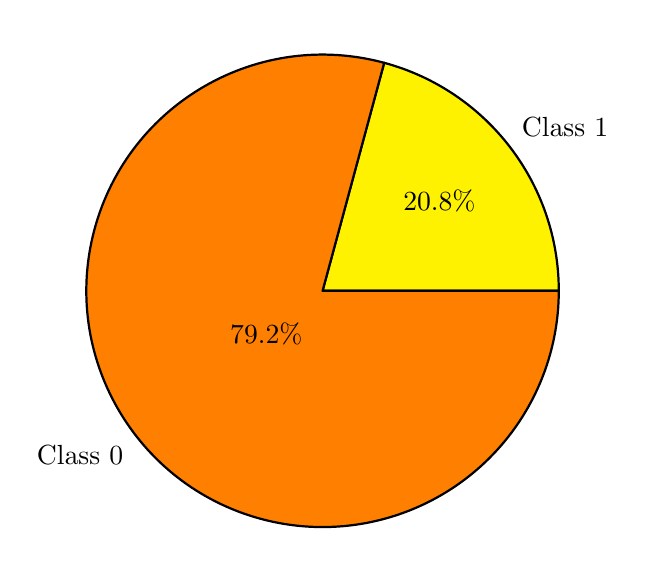
\begin{tikzpicture}
        \pie[color={yellow, orange}]{20.8/Class 1, 79.2/ Class 0}
    \end{tikzpicture}
\end{center}

\begin{center}
\textbf{Figure 1: Class Distribution}
\end{center}

This imbalance causes the classifier to not work properly due to less/more number of records supporting each case. This problem is solved by the inclusion of sampling methods. Sampling is done to solve data imbalance by creating or deleting records to compensate for the improper class distribution. Over all the observation is such that the model is bad at predicting flight delay. 

\bigbreak
\bigbreak
\bigbreak

The various over-sampling and under-sampling techniques are applied to each classifier to find the best fitting technique. The results are tabulated as follows. 

\begin{center}
\captionof{table}{Decision Tree} \label{tab:title} 
\begin{tabular}{ |p{2cm}|p{1cm}|p{2cm}|p{1cm}|p{1cm}|p{2cm}| }
 \hline
 Samplers & Class & Precision & Recall & f1 & Accuracy\\
 \hline
 SMOTE  & 1  & 0.67 & 0.70 & 0.68 & 0.86 \\
        & 0  & 0.92 & 0.91 & 0.91 &  \\
\hline
 Weighted Average & & 0.87 & 0.86 & 0.87 &  \\
 \hline
 \hline
 ADASYN   & 1  & 0.36 & 0.40 & 0.38 & 0.72 \\
          & 0  & 0.84 & 0.82 & 0.83 & \\
\hline
 Weighted Average & & 0.74 & 0.73 & 0.73 & \\
 \hline
 \hline
 Random Over Sampler  & 1  & 0.69 & 0.70 & 0.69 & 0.87\\
               & 0  & 0.92 & 0.92 & 0.92 & \\
\hline
 Weighted Average & & 0.87 & 0.87 & 0.87 & \\
 \hline
 \hline
 Near Miss  & 1  & 0.23 & 0.67 & 0.35 & 0.47\\
               & 0  & 0.83 & 0.42 & 0.56 & \\
\hline
 Weighted Average & & 0.70 & 0.47 & 0.51 & \\
 \hline
 \hline
 Random Under Sampler  & 1  & 0.50 & 0.80 & 0.62 & 0.79\\
               & 0  & 0.94 & 0.79 & 0.86 & \\
\hline
 Weighted Average & & 0.85 & 0.79 & 0.81 & \\
 \hline
\end{tabular}

\end{center}

From Table 5 we find that Random Over-Sampler and SMOTE have best values for f1-scores. The other techniques fail to compare with them and show poor performances in prediction.


\break
\begin{center}
\captionof{table}{Extra Trees} \label{tab:title} 
\begin{tabular}{ |p{2cm}|p{1cm}|p{2cm}|p{1cm}|p{1cm}|p{2cm}| }
 \hline
 Samplers & Class & Precision & Recall & f1 & Accuracy\\
 \hline
 SMOTE  & 1  & 0.80 & 0.73 & 0.76 & 0.90 \\
        & 0  & 0.93 & 0.95 & 0.94 &  \\
\hline
 Weighted Average & & 0.90 & 0.91 & 0.90 &  \\
 \hline
 \hline
 ADASYN   & 1  & 0.79 & 0.73 & 0.76 & 0.90 \\
          & 0  & 0.93 & 0.95 & 0.94 & \\
\hline
 Weighted Average & & 0.90 & 0.90 & 0.90 & \\
 \hline
 \hline
 Random Over Sampler  & 1  & 0.83 & 0.70 & 0.76 & 0.90\\
               & 0  & 0.92 & 0.96 & 0.94 & \\
\hline
 Weighted Average & & 0.90 & 0.91 & 0.90 & \\
 \hline
 \hline
 Near Miss  & 1  & 0.41 & 0.84 & 0.55 & 0.71\\
               & 0  & 0.94 & 0.68 & 0.79 & \\
\hline
 Weighted Average & & 0.83 & 0.72 & 0.74 & \\
 \hline
 \hline
 Random Under Sampler  & 1  & 0.67 & 0.81 & 0.73 & 0.87\\
               & 0  & 0.95 & 0.89 & 0.92 & \\
\hline
 Weighted Average & & 0.89 & 0.88 & 0.88 & \\
 \hline
\end{tabular}

\end{center}

The same trend observed in Table 5 arises in Table 6 as Random Over Sampler and SMOTE are found to show good performances in prediction of delays compared to others.

\break
\begin{center}
\captionof{table}{Gradient Boosting} \label{tab:title} 

\begin{tabular}{ |p{2cm}|p{1cm}|p{2cm}|p{1cm}|p{1cm}|p{2cm}| }
 \hline
 Samplers & Class & Precision & Recall & f1 & Accuracy\\
 \hline
 SMOTE  & 1  & 0.83 & 0.73 & 0.78 & 0.91 \\
        & 0  & 0.93 & 0.96 & 0.95 &  \\
\hline
 Weighted Average & & 0.91 & 0.91 & 0.9 &  \\
 \hline
 \hline
 ADASYN   & 1  & 0.80 & 0.75 & 0.77 & 0.90 \\
          & 0  & 0.93 & 0.95 & 0.94 & \\
\hline
 Weighted Average & & 0.91 & 0.91 & 0.91 & \\
 \hline
 \hline
 Random Over Sampler  & 1  & 0.73 & 0.79 & 0.76 & 0.89\\
               & 0  & 0.94 & 0.92 & 0.93 & \\
\hline
 Weighted Average & & 0.90 & 0.90 & 0.90 & \\
 \hline
 \hline
 Near Miss  & 1  & 0.45 & 0.83 & 0.58 & 0.74\\
               & 0  & 0.94 & 0.73 & 0.82 & \\
\hline
 Weighted Average & & 0.84 & 0.75 & 0.77 & \\
 \hline
 \hline
 Random Under Sampler  & 1  & 0.73 & 0.79 & 0.76 & 0.89\\
               & 0  & 0.94 & 0.92 & 0.93 & \\
\hline
 Weighted Average & & 0.90 & 0.89 & 0.90 & \\
 \hline
\end{tabular}

\end{center}

The similar trend observed in Tabel 5 and Table 6 arises here in Table 7 as Random Over Sampler and SMOTE Classifiers rank better than others in prediction.\\

Here since sampled and non sampled data have the same best f1-scores, sampling tends to be non-effective.
The conclusion from applying different sampling techniques would be that the different techniques tend to be less effective for the current data-set as they result in non reliable output.

The Gradient Boosting SMOTE sampled model is concluded to predict the chance of flight delay to a better extent than the other models. For the pipe-line output, the train and test sets are re-partitioned with training sets to be flights in the year 2016 and testing sets to be flights in the year 2017. The results of test set as predicted by the Gradient Boosting using SMOTE model is pipe-lined to the next module for prediction of flight delay minutes.

\clearpage

\section{Regression - Module 3}

The last module of the project deals with predicting the amount of delay occurred, in case of flight delay. The module implements a regression model to predict the necessary output. Since only delayed flights are to be considered, the rest flight details are removed from the set. The set is partitioned into train and test sets in a ratio 80:20. The module also makes use of the prediction from previous module's output of chance of flight delay for the year 2017 and predicts flight delay minutes.

    
\subsection{Metrics Used}
\begin{center}

Root mean squared error  \textbf{RMSE} = $\displaystyle\sqrt{\frac{1}{n}\sum_{t=1}^{n}e_t^2}$ \\
\bigbreak

Mean absolute error  \textbf{MAE} = $\displaystyle\frac{1}{n}\sum_{t=1}^{n}|e_t|$ \\
\bigbreak


R Squared \textbf{R2} = $\displaystyle\frac{Total Variation-Explained Variation}{Total Variation}$ \\
\end{center}
\bigbreak


\subsection{Analysis}

\subsubsection{Box plot: Arrival Delay Minutes}

\begin{center}
    
\begin{tikzpicture}
  \begin{axis}
    [
    ytick={1},
    yticklabels={Minutes},
    ]
    \addplot+[
    boxplot prepared={
      median=39,
      upper quartile=75.0,
      lower quartile=23.0,
      upper whisker=150.0,
      lower whisker=18.0
    },
    ] coordinates {};
  \end{axis}
\end{tikzpicture}

\end{center}

\begin{center}
    \textbf{Figure 2: Box Plot of Distribution of Arrival Delay Minutes}
\end{center}

From the box plot distribution we understand that the Inter Quartile range lies between 23 minutes and 75 minutes. This observation provides the fact that the data-set has delay minutes values more prominently  between the range of 23 and 75 minutes. In a practical approach, the model is trained to predict values primarily lying between the Inter Quartile Range. 

\subsubsection{Feature Selection : Embedded Methods}

Embedded methods are iterative in a sense that they take care of each iteration of the model's training process and carefully extracts those features which contribute the most to the training for a particular iteration. Regularization methods are the most commonly used embedded methods which penalize a feature given a coefficient threshold.
Here we will do feature selection using Lasso regularization. If the feature is irrelevant, lasso penalizes it’s coefficient and make it 0. Hence the features with coefficient = 0 are removed and the rest are taken.\\

Performing Lasso Regression the model picked 9 features to be important and discarded 13 other features to be not important. The feature importance plot is as shown below

\begin{center}
  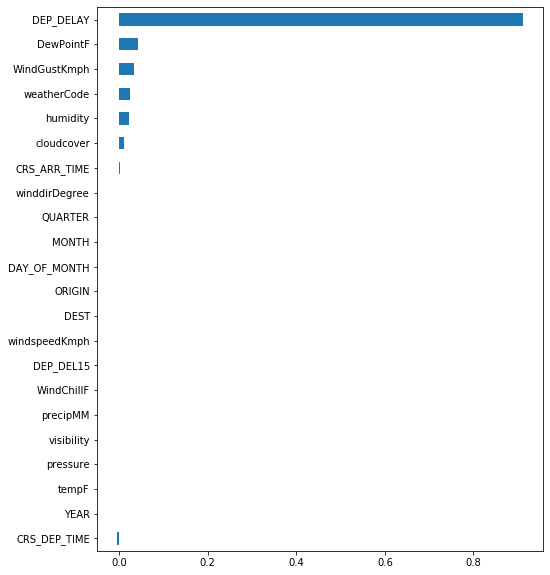
\includegraphics[width=0.7\textwidth]{bar.png}{H}
  \bigbreak
  \textbf{Figure 3: Feature Importance Using Lasso Model}
\end{center}

From figure 3 we observe that \textbf{Departure delay Minutes} feature denoting the number of minutes delayed during departure, \textbf{Dew Point} feature denoting the temperature to which air must be cooled to become saturated with water vapor and \textbf{Wind Gust speed} feature denoting the sudden increase of wind speed are the features that contribute the most in predicting \textbf{Arrival Delay Minutes}.

\clearpage

\subsubsection{Correlation : SNS Heat Map}

Filter method is used to find relevance between features using correlation matrix by implementing Pearson correlation. The correlation matrix heat map for \textbf{Arrival Delay Minutes} feature with other features of the data-set is as follows.

\begin{center}
  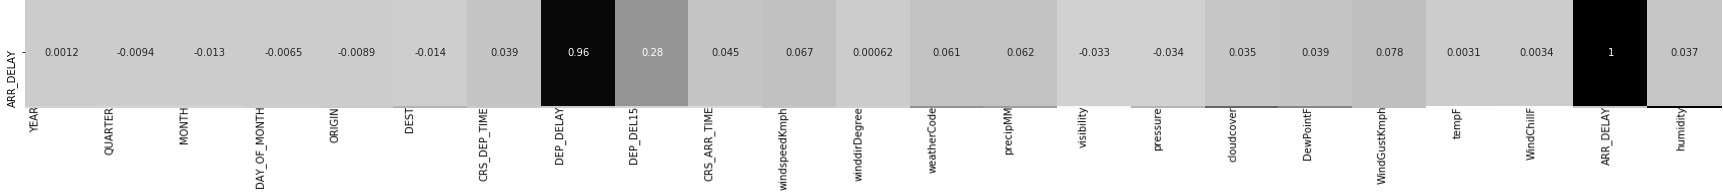
\includegraphics[width=1\textwidth]{final.jpg}
   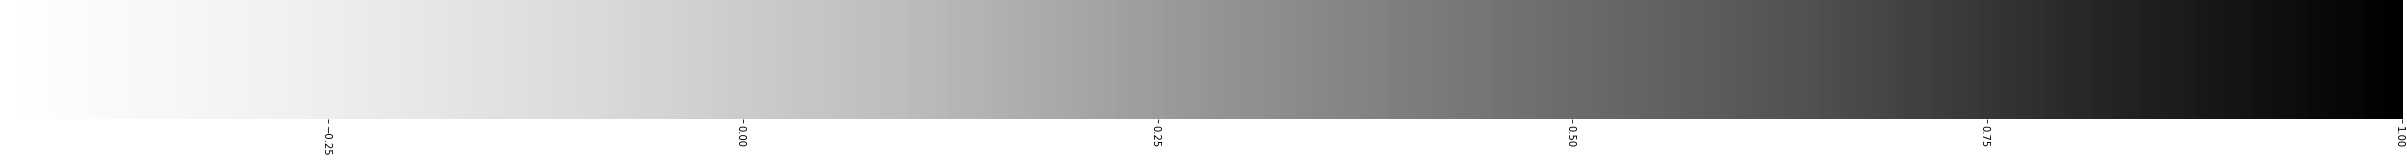
\includegraphics[width=1\textwidth]{3.png}
  \bigbreak
  \textbf{Figure 4: SNS Heat Map}
\end{center}

From the heat map we observe the following features to be of maximum relevance to \textbf{Arrival Delay minutes}. \\

\textbf{Departure delay minutes} feature denoting the number of minutes delayed during departure. \textbf{Departure delay} feature indicating whether a flight has been delayed or not and \textbf{Wind Speed} denoting the speed of wind in Kmph.

\subsection{Tabulated Results}


The results of different models that predicted flight delay minutes for flight delays from actual data-set are tabulated as follows. 
\begin{center}
\captionof{table}{Regression model scores - Actual Delays} \label{tab:title} 
\begin{tabular}{ |c|c|c|c| } 
 \hline
 \textbf{Model} & \textbf{MAE} & \textbf{RMSE} & \textbf{R2} \\
 \hline
 Linear Regression & 12.34 & 17.77 & 0.94 \\ 
 \hline
 XGBoost & 11.63 & 16.88 & 0.94 \\
 \hline
 Extra Trees & 11.85 & 16.92 & 0.94 \\
 \hline
 Decision Trees & 16.59 & 24.13 & 0.88 \\
 \hline
\end{tabular}
\end{center}
\bigbreak

The results of different models that predicted flight delay minutes for flight delays predicted by module 2 are tabulated as follows.

\begin{center}
\captionof{table}{Regression model scores - Predicted Delays} \label{tab:title} 
\begin{tabular}{ |c|c|c|c| } 
 \hline
 \textbf{Model} & \textbf{MAE} & \textbf{RMSE} & \textbf{R2} \\
 \hline
 Linear Regression & 10.78 & 15.11 & 0.88 \\ 
 \hline
 XGBoost & 10.55 & 14.81 & 0.89 \\
 \hline
 Extra Trees & 10.37 & 14.48 & 0.89 \\
 \hline
 Decision Trees & 14.86 & 20.66 & 0.79 \\
 \hline
\end{tabular}
\end{center}
\bigbreak

From the table 8 and table 9 we observe that the models predict values with less errors from pipe-line output obtained from previous model than the original data-set.

\subsection{Post Regression Analysis}

\subsubsection{Box plot: Predicted Arrival Delay Minutes}

\begin{center}
    
\begin{tikzpicture}
  \begin{axis}
    [
    ytick={1},
    yticklabels={Minutes},
    ]
    \addplot+[
    boxplot prepared={
      median=35,
      upper quartile=69.0,
      lower quartile=24.0,
      upper whisker=130.0,
      lower whisker=18.0
    },
    ] coordinates {};
  \end{axis}
\end{tikzpicture}

\end{center}

\begin{center}
    \textbf{Figure 5: Box Plot of Distribution of Predicted Arrival Delay Minutes}
\end{center}

From figure 5 we observe that the Inter Quartile Range lies between 24 minutes and 69 minutes. The range is maintained the same to an extent as in before prediction with consideration of figure 2. Thereby the trained model predicts delay minutes primarily in the Inter Quartlie Range.

\subsubsection{Feature Importance}

The Feature Importance concept from the tree models post regression is able to perform the ranking of features based on importance of features to the machine learning model. 
Upon ranking and observation, we infer that the \textbf{Scheduled departure time} denoting the scheduled time of departure of flight, \textbf{Departure delay} indicating whether a flight is delayed during departure or not and \textbf{Departure delay minutes} denoting the number of minutes flight has been delayed during departure are the set of features that act as most important to the model in predicting delay minutes.

\section{Conclusion}

 The first stage deals with classifying flights to be delayed or not. Due to data-imbalance, sampling techniques are employed to compensate for the improper data distribution. Sampling does not however solve the situation and is ineffective in predicting flight delay for the given data-set. Hence by consideration of better scores among all other classifiers implemented, the \textbf{Gradient Boosting Classifier} sampled under SMOTE proved better with an accuracy of 91 \%\/. The follow up module worked on predicting the amount of delay for delayed flights by running different regression algorithms. Among the various regressors considered, the \textbf{XGBoost Regressor} resulted in the most efficient output with minimum MAE (11.63) and RMSE (16.88) score. The two-stage predictive machine learning model is implemented on basis of above conclusion of techniques to work efficiently for the given problem statement.

\end{document}
